\chapter{Experiments and Improvements}\label{experiments_and_improvements}

In order to enhance the proposed model, we employed different strategies for finding improvements: \begin{itemize}
	\item We tried smaller and faster networks that are data efficient to optimize the current architecture.
	\item We tested more powerful architectures that proved to be successful (Transformers) in the case of natural language processing.
	\item We extended a model with an additional module for handling other musical elements: dynamics.\end{itemize}
	
Let us present results of these experiments.

\section{Transformers}

\emph{Transformers} are a class of neural network architectures introduced by Vaswani et al. in the landmark paper \emph{Attention Is All You Need} \cite{Vaswani2017}. Originally developed for natural language processing (NLP), have since become versatile and powerful framework for modeling sequential data across numerous other fields, including image processing \cite{Dosovitskiy2020}, audio generation \cite{Borsos2023} and even symbolic music analysis \cite{Zhu2021}.

\begin{figure}[ht!]
\centering
\begin{tikzpicture}
    \tikzset{block/.style={fill=gray!20, text width=3.5cm, draw=black, thick, text centered, align=center, rounded corners, minimum height=1.5em, minimum width=3.5cm}}
    \tikzset{input/.style={fill=gray!30, text width=3.5cm, draw=black, thick, text centered, rounded corners, minimum height=1.5em, minimum width=3.5cm}}
    \tikzset{operation/.style={draw, circle, thick, minimum size=0.75cm}}
    \tikzset{arrowstyle/.style={-{Latex[length=3mm]}}}

    \node (inputs) at (0, 1.5) {Inputs};
    \node (outputs) at (6, 1.5) {Shifted Outputs};

    \node[input] (input_embed) at (0, 0) {Input Embedding};
    \node[block] (pos_encoding) at (-3, -1.2) {Positional \\ Encoding};
    \node[operation] (add1) at (0, -1.2) {$+$};

    \node[block] (multihead1) at (0, -3.25) {Multi-Head \\ Attention};
    \node[block] (add_norm1) at (0, -4.5) {Add \& Norm};
    \node[block] (ffn1) at (0, -6.25) {Feed \\ Forward};
    \node[block] (add_norm2) at (0, -7.5) {Add \& Norm};

    \draw[rounded corners, thick] (-2.75, -2) rectangle (2.75, -8.25) node[pos=0.5, xshift=-3.1cm] {$N \times \;$};

    \node[input] (output_embed) at (6, 0) {Output Embedding};
    \node[block] (pos_encoding_dec) at (9, -1.2) {Positional \\ Encoding};
    \node[operation] (add2) at (6, -1.2) {$+$};

    \node[block] (masked_mha) at (6, -3.25) {Masked Multi-Head \\ Attention};
    \node[block] (add_norm_dec1) at (6, -4.5) {Add \& Norm};
    \node[block] (mha_dec) at (6, -6.40) {Multi-Head \\ Attention};
    \node[block] (add_norm_dec2) at (6, -7.50) {Add \& Norm};
    \node[block] (ffn2) at (6, -9.25) {Feed \\ Forward};
    \node[block] (add_norm_dec3) at (6, -10.50) {Add \& Norm};

    \draw[rounded corners, thick] (3.25, -2) rectangle (8.75, -11.25) node[pos=0.5, xshift=3.1cm] {$\, \times N$};

    \node[block] (linear) at (6, -12.2) {Linear};
    \node[block] (softmax) at (6, -13.6) {Softmax};
    \node (output_probs) at (6, -15.1) {Output Probabilities};

    \draw[arrowstyle] (inputs.south) -- (input_embed.north);
    \draw[arrowstyle] (input_embed.south) -- (add1.north);
    \draw[arrowstyle] (pos_encoding.east) -- (add1.west);
    \draw[arrowstyle] (add1) -- (multihead1);
    \draw[arrowstyle] (multihead1) -- (add_norm1);
    \draw[arrowstyle] (add_norm1) -- (ffn1);
    \draw[arrowstyle] (ffn1) -- (add_norm2);

    \draw[arrowstyle] (outputs.south) -- (output_embed.north);
    \draw[arrowstyle] (output_embed.south) -- (add2.north);
    \draw[arrowstyle] (pos_encoding_dec.west) -- (add2.east);
    \draw[arrowstyle] (add2) -- (masked_mha);
    \draw[arrowstyle] (masked_mha) -- (add_norm_dec1);
    \draw[arrowstyle] (mha_dec) -- (add_norm_dec2);
    \draw[arrowstyle] (add_norm_dec2) -- (ffn2);
    \draw[arrowstyle] (ffn2) -- (add_norm_dec3);
    \draw[arrowstyle] (add_norm_dec3) -- (linear);
    \draw[arrowstyle] (linear) -- (softmax);
    \draw[arrowstyle] (softmax) -- (output_probs);

    \draw[arrowstyle] (add_norm2.east) -| ++(0.325, 0) |- ++(0, 2.05) -| ($(mha_dec.north) - (1.0, 0.0)$);
    \draw[arrowstyle] (add_norm2.east) -| ++(0.325, 0) |- ++(0, 2.05) -| (mha_dec.north);

    \draw[arrowstyle] (0, -2.25) -| ++(-2.325,0) |- (add_norm1.west);
    \draw[arrowstyle] (0, -5.25) -| ++(-2.325,0) |- (add_norm2.west);

    \draw[arrowstyle] (0, -2.35) -| ++(-1.0,0) -- ($(multihead1.north) - (1.0, 0.0)$);
    \draw[arrowstyle] (0, -2.35) -| ++(1.0,0) -- ($(multihead1.north) + (1.0, 0.0)$);

    \draw[arrowstyle] (6, -2.35) -| ++(-1.0,0) -- ($(masked_mha.north) - (1.0, 0.0)$);
    \draw[arrowstyle] (6, -2.35) -| ++(1.0,0) -- ($(masked_mha.north) + (1.0, 0.0)$);

    \draw[arrowstyle] (add_norm_dec1) -- (6, -5.25) -| ++(1.0,0) -- ($(mha_dec.north) + (1.0, 0.0)$);

    \draw[arrowstyle] (6, -2.25) -| ++(2.325,0) |- (add_norm_dec1.east);
    \draw[arrowstyle] (6, -5.25) -| ++(2.325,0) |- (add_norm_dec2.east);
    \draw[arrowstyle] (6, -8.25) -| ++(2.325,0) |- (add_norm_dec3.east);

\end{tikzpicture}
\caption[The Transformer architecture.]{The Transformer architecture \cite{Vaswani2017}.}
\end{figure}

The key innovation in Transformers is the \emph{self-attention} mechanism, which enables the model to weigh the relevance of each part of an input sequence relative to other parts, regardless of their distance from each other in the sequence. Unlike recurrent neural networks, which process data sequentially and can struggle with long-range dependencies, Transformers use that mechanism to directly model these dependencies in parallel.

As the authors state at the end of the paper \cite{Liu2022}: \begin{quote}Possible next steps include investigating more powerful model architectures such as the Transformer.\end{quote} We analyzed various setups involving Transformer and attention mechanisms, preserving the training and evaluation setup.

\subsection{Vanilla Transformer}

We tested the vanilla architecture of the Transformer model, limited to the encoder only\footnote{There is no decoding in the transcription task.}. As a rule of thumb, we decided to keep the model size comparable to the original network. Different number of embedding sizes have been employed, ranging from $128$ to $512$. 

As Transformers are primarily used for sequential discrete data, we used an additional encoding scheme with discretized note durations and note velocities. The note durations have been encoded using the same number of features as onsets, and the velocity, as a minor parameter, has been reduced to 8 discrete categories.

\begin{figure}[ht!]
\centering
\begin{tabular}{cc}a)
\scalebox{0.8}{
\begin{tikzpicture}
    \tikzset{block/.style={fill=gray!20, text width=3.5cm, draw=black, thick, text centered, align=center, rounded corners, minimum height=1.5em, minimum width=3.5cm}}
    \tikzset{input/.style={fill=gray!30, text width=3.5cm, draw=black, thick, text centered, rounded corners, minimum height=1.5em, minimum width=3.5cm}}
    \tikzset{operation/.style={draw, circle, thick, minimum size=0.75cm}}
    \tikzset{arrowstyle/.style={-{Latex[length=3mm]}}}

    \node (inputs) at (0, 1.5) {Inputs};
    \node[input] (input_embed) at (0, 0) {Input Embedding};
    \node[block] (pos_encoding) at (-3, -1.2) {Positional \\ Encoding};
    \node[operation] (add) at (0, -1.2) {$+$};
    \node[block] (transformer) at (0, -2.7) {Transformer Encoder};
    \node[input] (linear) at (0, -4.2) {Linear};
    \node (output) at (0, -5.7) {Output Probabilities};

    \draw[arrowstyle] (inputs.south) -- (input_embed.north);
    \draw[arrowstyle] (input_embed.south) -- (add.north);
    \draw[arrowstyle] (pos_encoding.east) -- (add.west);
    \draw[arrowstyle] (add) -- (transformer);
    \draw[arrowstyle] (transformer) -- (linear);
    \draw[arrowstyle] (linear) -- (output);

\end{tikzpicture}
} & b)
\scalebox{0.8}{
    \begin{tikzpicture}
    \tikzset{block/.style={fill=gray!20, text width=3.5cm, draw=black, thick, text centered, align=center, rounded corners, minimum height=1.5em, minimum width=3.5cm}}
    \tikzset{input/.style={fill=gray!30, text width=3.5cm, draw=black, thick, text centered, rounded corners, minimum height=1.5em, minimum width=3.5cm}}
    \tikzset{embedding/.style={fill=gray!40, text width=1.5cm, draw=black, thick, text centered, rounded corners, minimum height=1.5em, minimum width=1.5cm}}
    \tikzset{operation/.style={draw, circle, thick, minimum size=0.75cm}}
    \tikzset{arrowstyle/.style={-{Latex[length=3mm]}}}

    \node (pitch) at (-3.0, 1.5) {Pitch};
    \node (onset) at (-1.0, 1.5) {Onset};
    \node (duration) at (1.0, 1.5) {Duration};
    \node (velocity) at (3.0, 1.5) {Velocity};
    \node[embedding] (pitch_embed) at (-3.0, 0) {Embed.};
    \node[embedding] (onset_embed) at (-1.0, 0) {Embed.};
    \node[embedding] (duration_embed) at (1.0, 0) {Embed.};
    \node[embedding] (velocity_embed) at (3.0, 0) {Embed.};
    \node[block] (pos_encoding) at (-3, -2.7) {Positional \\ Encoding};
    \node[operation] (add1) at (0, -1.2) {$+$};
    \node[operation] (add2) at (0, -2.7) {$+$};
    \node[block] (transformer) at (0, -4.2) {Transformer Encoder};
    \node[input] (linear) at (0, -5.7) {Linear};
    \node (output) at (0, -7.2) {Output Probabilities};

    \draw[arrowstyle] (pitch.south) -- (pitch_embed.north);
    \draw[arrowstyle] (onset.south) -- (onset_embed.north);
    \draw[arrowstyle] (duration.south) -- (duration_embed.north);
    \draw[arrowstyle] (velocity.south) -- (velocity_embed.north);
    \draw[arrowstyle] (pitch_embed.south) |- (add1.west);
    \draw[arrowstyle] (onset_embed.south) |- (add1.west);
    \draw[arrowstyle] (duration_embed.south) |- (add1.east);
    \draw[arrowstyle] (velocity_embed.south) |- (add1.east);
    \draw[arrowstyle] (pos_encoding.east) -- (add2.west);
    \draw[arrowstyle] (add1) -- (add2);
    \draw[arrowstyle] (add2) -- (transformer);
    \draw[arrowstyle] (transformer) -- (linear);
    \draw[arrowstyle] (linear) -- (output);

\end{tikzpicture}
}
\end{tabular}
\caption[The Transformer Encoder block.]{The Transformer Encoder block: a) default encoding, b) feature embedding. The positional encoding is optional.}
\end{figure}

For the training, we decreased the learning rate from the default value \num{1e-3} to \num{1e-4} and we set a warmup of 2500 steps. Variants without positional encoding have been tested as well\footnote{Language models have been reported to learn comparably good without positional encodings \cite{Haviv2022}.}.

We stick to the default \texttt{pytorch} implementation of the Transformer encoder layer.

\subsection{Results}

In general, Transformers didn't perform as good as the original model. Positional encoding worsened the results in almost all cases.

We present various setups for all submodels: the beat model, the hand part model, the key and time signature models.

\subsection{Beat Model}


\subsection{Hand Part Model}

The hand part model

\subsection{Key Signature Model}

\subsection{Time Signature Model}


\section{Attention}

In subsequent experiments we stepped out from the full Transformer for attention mechanism only. We wanted to check whether access to the entire tensor sequence is beneficial for the transcription task.

We hypothesize that Transformer architecture could outperform the proposed network but in a data-abundant scenario, but the entire dataset is still too small and needs more data-efficient models.

Moreover local features distilled from convolutional neural networks are sufficient most of the time. 
\missing

% We hypothesize that Transformer architecture could outperform the proposed network but in a data-abundant scenario, but the entire dataset is still too small and needs more data-efficient models.

% Moreover, the models' assignment heavy rely on small context of the piece. In other words, musical information that lies far apart from notes is not particularly useful for the inference.

\section{Temporal Convolutional Network}

Classical convolutional networks usually have a rather small receptive field\footnote{\emph{Receptive field} can be understood as the size of the region in the input data that produces a feature \cite{Araujo2019}. For a point on a grid, these and only these parts in that region are accessible by the network.}, and the canonical way to enlarge the size is to stack several layers of the network. As the input sequence can be very large, covering greater portions of data requires more model parameters, which at some point may yield too complex architecture for a given data scenario.

\subsection{Dilated Convolution}

To keep the size of the model small, one could use a \emph{dilated convolution}, which expands the receptive field by spacing out the kernel element with gaps, called \emph{dilation rates}.

\begin{figure}[ht!]
\centering
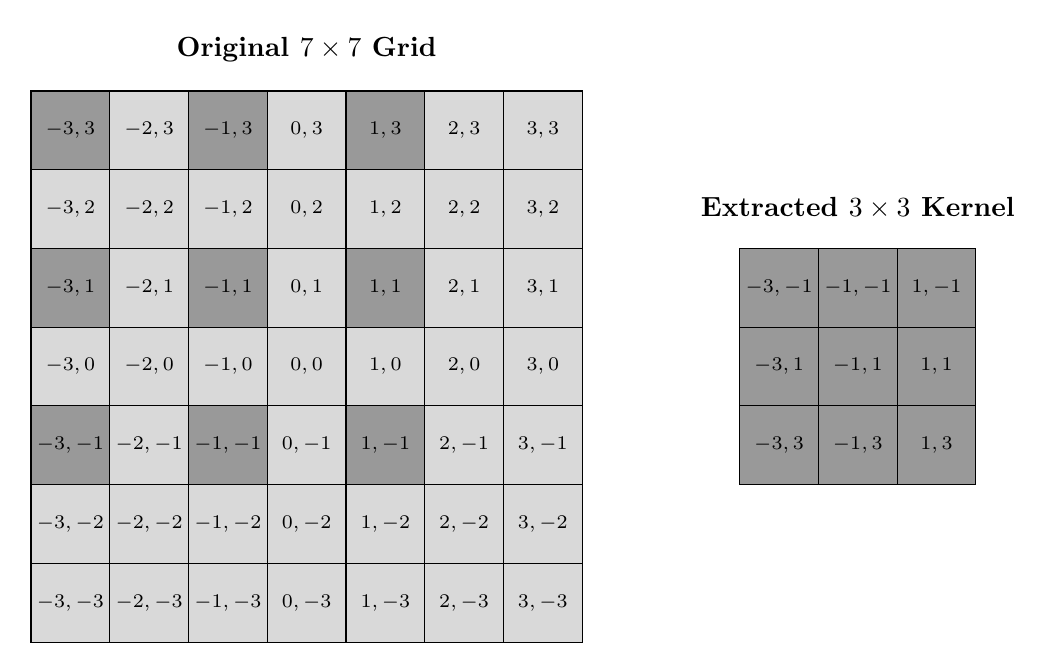
\begin{tikzpicture}
    \foreach \x in {-3,-2,-1,0,1,2,3} {
        \foreach \y in {-3,-2,-1,0,1,2,3} {
            \fill[gray!30] (\x, \y) rectangle (\x+1, \y+1);
            \draw[black] (\x, \y) rectangle (\x+1, \y+1);
        }
    }

    \fill[gray!80] (-3, 3) rectangle (-2, 4);
    \fill[gray!80] (-1, 3) rectangle (0, 4);
    \fill[gray!80] (1, 3) rectangle (2, 4);
    \fill[gray!80] (-3, 1) rectangle (-2, 2);
    \fill[gray!80] (-1, 1) rectangle (0, 2);
    \fill[gray!80] (1, 1) rectangle (2, 2);
    \fill[gray!80] (-3, -1) rectangle (-2, 0);
    \fill[gray!80] (-1, -1) rectangle (0, 0);
    \fill[gray!80] (1, -1) rectangle (2, 0);
    \draw[black] (-3, 3) rectangle (-2, 4);
    \draw[black] (-1, 3) rectangle (0, 4);
    \draw[black] (1, 3) rectangle (2, 4);
    \draw[black] (-3, 1) rectangle (-2, 2);
    \draw[black] (-1, 1) rectangle (0, 2);
    \draw[black] (1, 1) rectangle (2, 2);
    \draw[black] (-3, -1) rectangle (-2, 0);
    \draw[black] (-1, -1) rectangle (0, 0);
    \draw[black] (1, -1) rectangle (2, 0);

    \foreach \x in {-3,-2,-1,0,1,2,3} {
        \foreach \y in {-3,-2,-1,0,1,2,3} {
            \node[font=\scriptsize] at (\x+0.5, \y+0.5) {\scriptsize $\x,\y$};
        }
    }

    \foreach \i [count=\ix from -1] in {-3,-1,1} {
        \foreach \j [count=\jx from -1] in {3,1,-1} {
            \fill[gray!80] (7+\ix, \jx) rectangle (8+\ix, \jx+1);
            \draw[black] (7+\ix, \jx) rectangle (8+\ix, \jx+1);
            \node[font=\scriptsize] at (7.5+\ix, \jx+0.5) {\scriptsize $\i,\j$};
        }
    }

    \node[above] at (0.5, 4.25) {\textbf{Original $7 \times 7$ Grid}};
    \node[above] at (7.5, 2.25) {\textbf{Extracted $3 \times 3$ Kernel}};
\end{tikzpicture}

\caption[Dilated convolution.]{Dilated convolution with kernel size $k = 3$ and dilation rate $d = 2$, illustrated on the $(-1, 1)$ point on a $7 \times 7$ grid.}
\end{figure}

Dilated convolutional layers increase the receptive field of the network exponentially with linear parameter accretion. 

While the idea can be traced back to wavelet decompositions from 1989 \cite{Holschneider1989}, the rediscovery of the method in the machine learning field can be attributed to Chen et al. \cite{Chen2015}.

\subsection{Temporal Convolutional Network}

Temporal Convolutional Network (TCN), introduced by \cite{Colin2016}, leverage the idea of dilated convolutions, to cover varied regions of data in a hierarchical way. The network consists of layers of dilated convolutions, where the dilation rate increases exponentially, starting from $d = 1, 2, 4$ and so on.

For sequential or time-series data, this structure strikes a balance between capturing both short-term and long-term dependencies. While TCNs can look ahead in time, they exhibit behavior similar to recurrent networks.

They are several advantages of using TCNs over recurrent networks: \begin{itemize}
	\item Recurrent networks suffer from inability to parallelize computation, as the result of next state is dependent on the previous one. This is no longer a problem of convolutional networks. The TCNs can be trained much faster.
	\item Recurrent networks need careful architecture adjustments to capture long-term relationships. Dilated convolutions allows to directly control the range of the field.
	\item The training of convolutional networks is usually stable. Recurrent networks are reported to be unstable during training. One of the reasons behind that phenomenon is the problem of vanishing/exploding gradients. However, gated recurrent units mitigate some of these issues. 
\end{itemize}

In some cases, these advantages come without sacrificing the performance. In the next sections we are going to show that indeed is the case for certain transcription subtasks. Before that, let us provide more details on the exact model structure.

\subsection{Model Architecture}

Since the musical features are not spatial, the convolutions are one-dimensional. We used the TCN variant of the kernel size $9$, and dilation rates $1$, $2$ and $4$. The receptive field $r$ can be calculated as the following sum: \[r = 1 + \sum_{i=1}\left(k_i - 1\right)\cdot d_i\] where $k_i$ is the kernel size, and $d_i$ is the dilation rate at $i$-th layer. Here, the receptive field after $3$ layers is $r_3 = 57$. See Figure \ref{temporal_convolutional_network} for the architecture layout.

\begin{figure}[ht!]
\centering
\begin{tikzpicture}
    \tikzset{layer1/.style={fill=gray!10, draw=gray, thick, text centered}}
    \tikzset{layer2/.style={fill=gray!30, draw=gray, thick, text centered}}
    \tikzset{operation/.style={draw, circle, thick, minimum size=0.75cm}}
    \tikzset{arrowstyle/.style={-{Latex[length=3mm]}}}

    \fill[fill=gray!50, fill opacity=0.5, draw=gray, thick, line width=2pt] (0.0, -2.0) rectangle (12.0, 7.0);
    \fill[fill=white!50, fill opacity=1.0, draw=black, thick, line width=1pt] (0.5, 0.0) rectangle (10.5, 6.5);
    \fill[fill=white!50, fill opacity=1.0, draw=black, thick, line width=1pt] (1.0, -0.5) rectangle (11.0, 6.0);
    \fill[fill=white!50, fill opacity=1.0, draw=black, thick, line width=1pt] (1.5, -1.0) rectangle (11.5, 5.5);

    \draw (6.5, 9.00) node (note_sequence) {Note sequence};
    \draw (6.5, 8.00) node[layer1] (embedding) {Linear};
    \draw (4.0, 4.50) node[layer1] (layerA1) {Dilated Convolutional};
    \draw (4.0, 3.50) node[layer1] (layerA2) {ReLU};
    \draw (4.0, 2.50) node[layer1] (layerA3) {Dropout};
    \draw (4.0, 1.50) node[layer1] (layerA4) {Dilated Convolutional};
    \draw (6.5, 0.75) node[operation] (add) {$+$};
    \draw (6.5, -0.50) node[layer2] (layerA5) {Layer Normalization};
    \draw[anchor=south, inner sep=2pt] (6.5, -2.0) node (outputA) {To the next convolutional layer};

    \draw (6.5, -3.00) node[layer1] (output) {Linear};

    \node[anchor=south west, inner sep=2pt] at (0.2, -1.8) {TCNBlock};

    \node[anchor=north west, inner sep=2pt] at (1.55, 5.45) {\small{9, 1, 256}};
    \node[anchor=north west, inner sep=2pt] at (1.05, 5.95) {\small{9, 2, 256}};
    \node[anchor=north west, inner sep=2pt] at (0.55, 6.45) {\small{9, 4, 256}};
    \node[anchor=north west, inner sep=2pt] at (0.05, 6.95) {\small{kernel size, dilation, hidden size}};

    \draw[arrowstyle] (note_sequence.south) to (embedding.north);
    \draw[arrowstyle] (embedding.south) -| ++(0.0, -2.5) -| (layerA1.north);
    \draw[arrowstyle] (embedding.south) -| ++(0.0, -2.5) -| ++(2.5, 0.0) |- (add.east);
    \draw[arrowstyle] (layerA1.south) to (layerA2.north);
    \draw[arrowstyle] (layerA2.south) to (layerA3.north);
    \draw[arrowstyle] (layerA3.south) to (layerA4.north);
    \draw[arrowstyle] (layerA4.south) |- (add.west);
    \draw[arrowstyle] (add.south) to (layerA5.north);
    \draw[arrowstyle] (layerA5.south) to (outputA.north);
    \draw[arrowstyle] (outputA.south) to (output.north);
\end{tikzpicture}

\caption[The Temporal Convolutional Block.]{The Temporal Convolutional Block.}
\label{temporal_convolutional_network}
\end{figure}

We considered two variants of the model: with $128$ and $256$ number of filters per convolutional layer.

The training/evaluation setup remained exactly the same.

\subsection{Results}

The experiments conducted using TCNs shows that, for certain models, the networks achieved comparable of superior results while having smaller number of parameters, and, due to the nature of the architecture, training much faster than recurrent networks. 

\subsubsection{Beat Model}

The neural network of the beat quantization model has been replaced by TCNn. The original model performed better than the both TCN variants, however the bigger TCN model performed only slightly worse than the original model.

\begin{table}[ht!]
\centering
\begin{tabular}{cc|ccc}
    \multicolumn{2}{c|}{\textbf{Model}} & \textbf{Original} & \textbf{TCN 128} & \textbf{TCN 256} \\
    \multicolumn{2}{c|}{\textbf{Parameters}} & 27.5 M & 7.6 M & 10.9 M \\\hline
    \multirow{4}{*}{Beats}     & Accuracy    & $\mathbf{0.880}$ & $ $ & $0.848$          \\
    & Precision   & $\mathbf{0.879}$ & $ $ & $0.832$          \\
    & Recall      & $\mathbf{0.873}$ & $ $ & $0.831$          \\
    & $F_1$ score & $\mathbf{0.864}$ & $ $ & $0.819$          \\\hline
    \multirow{4}{*}{Downbeats} & Accuracy    & $\mathbf{0.853}$ & $ $ & $\mathbf{0.867}$ \\
    & Precision   & $0.622$          & $ $ & $0.660$ \\
    & Recall      & $\mathbf{0.467}$ & $ $ & $0.568$          \\
    & $F_1$ score & $\mathbf{0.508}$ & $ $ & $0.577$          \\\hline
    \multirow{4}{*}{Beats}     & Accuracy    & $\mathbf{0.869}$ & $0.823$ & $0.851$          \\
    & Precision   & $\mathbf{0.859}$ & $0.795$ & $0.842$          \\
    & Recall      & $\mathbf{0.884}$ & $0.848$ & $0.847$          \\
    & $F_1$ score & $\mathbf{0.859}$ & $0.802$ & $0.831$          \\\hline
    \multirow{4}{*}{Downbeats} & Accuracy    & $\mathbf{0.860}$ & $0.854$ & $\mathbf{0.860}$ \\
    & Precision   & $0.665$          & $0.640$ & $\mathbf{0.704}$ \\
    & Recall      & $\mathbf{0.486}$ & $0.453$ & $0.406$          \\
    & $F_1$ score & $\mathbf{0.545}$ & $0.513$ & $0.494$          \\\hline
    \multicolumn{2}{c|}{Meter} & $\mathbf{0.579}$ & $0.537$ & $0.576$ \\
\end{tabular}

\caption[Temporal Convolutional Network results for the beat model.]{Temporal Convolutional Network results for the beat model.}
\label{beat_tcn}
\end{table}

Increasing the number of layers not only didn't improve the results but worsened the quality of the model.

The dynamic programming algorithm for out-of-note beat prediction has been left intact.

\subsubsection{Hand Part Model}

The TCN hand part model comparable results for both two variants, while having a much smaller and faster network.

\begin{table}[ht!]
\centering
\begin{tabular}{c|ccc}
    \textbf{Model}      & \textbf{Original} & \textbf{TCN 128} & \textbf{TCN 256} \\
    \textbf{Parameters} & 10.5 M           & 954 K            & 3.7 M            \\\hline
    Accuracy            & $\mathbf{0.956}$ & $0.917$          & $0.919$          \\
    Precision           & $0.851$          & $\mathbf{0.908}$ & $\mathbf{0.908}$ \\
    Recall              & $0.848$          & $0.865$          & $\mathbf{0.872}$ \\
    $F_1$ score         & $0.842$          & $0.885$          & $\mathbf{0.888}$ \\
    Voice separation    & $\mathbf{0.820}$ & $0.805$          & $0.806$          \\
\end{tabular}
\caption[Temporal Convolutional Network results for the hand part model.]{Temporal Convolutional Network results for the hand part model.}
\label{hand_part_tcn}
\end{table}

This shows no strong benefits of using recurrent networks in the case of hand part assignment.

\subsubsection{Key Signature Model}

The key signature model based on TCNs was not on par with the original model. The convolutional model struggled especially with rarer key signatures, which is visible by the discrepancy between macro and weighted metrics. 

\begin{table}[ht!]
\centering
\begin{tabular}{cc|ccc}
    \multicolumn{2}{c|}{\textbf{Model}} & \textbf{Original} & \textbf{TCN 128} & \textbf{TCN 256} \\
    \multicolumn{2}{c|}{\textbf{Parameters}} & 10.5 M & 955 K & 3.7 M \\\hline
    \multirow{3}{*}{Macro}    & Precision   & $\mathbf{0.812}$ & $0.307$          & $0.351$ \\
    & Recall      & $\mathbf{0.789}$ & $0.239$          & $0.284$ \\
    & $F_1$ score & $\mathbf{0.787}$ & $0.260$          & $0.307$ \\\hline
    \multirow{3}{*}{Weighted} & Precision   & $0.924$          & $\mathbf{0.954}$ & $0.951$ \\
    & Recall      & $\mathbf{0.898}$ & $0.673$          & $0.682$ \\
    & $F_1$ score & $\mathbf{0.896}$ & $0.771$          & $0.777$ \\\hline
    \multicolumn{2}{c|}{Harmony} & $\mathbf{0.972}$ & $0.878$ & $0.834$ \\
\end{tabular}

\caption[Temporal Convolutional Network results for the key signature model.]{Temporal Convolutional Network results for the key signature model.}
\label{key_signature_tcn}
\end{table}

Variants with more layers didn't improve the quality of the model.

\subsubsection{Time Signature Model}

The second version of the model consisted only on convolutional layers, without GRUs. The TCN architecture outperformed this model greatly.

\begin{table}[ht!]
\centering
\begin{tabular}{c|ccc}
    \textbf{Model}      & \textbf{Original} & \textbf{TCN 128} & \textbf{TCN 256} \\
    \textbf{Parameters} & 676 K             & 954 K            & 3.7 M            \\\hline
    Accuracy            & $0.560$           & $\mathbf{0.612}$ & $0.575$          \\
    Precision           & $\mathbf{0.315}$  & $0.280$          & $0.261$          \\
    Recall              & $0.230$           & $\mathbf{0.236}$ & $0.249$          \\
    $F_1$ score         & $\mathbf{0.258}$  & $0.248$          & $0.253$          \\\hline
    Accuracy            & $0.552$           & $0.655$          & $\mathbf{0.793}$ \\
    Precision           & $0.444$           & $0.625$          & $\mathbf{0.750}$ \\
    Recall              & $0.333$           & $0.417$          & $\mathbf{0.750}$ \\
    $F_1$ score         & $0.381$           & $0.500$          & $\mathbf{0.750}$ \\
\end{tabular}
\caption[Temporal Convolutional Network results for the time signature model.]{Temporal Convolutional Network results for the time signature model.}
\label{time_signature_tcn}
\end{table}

As in the case of ablation studies, the time signature model does not affect the MV2H metric.

\section{Dynamics}

\missing

\begin{figure}[!ht]
\centering
\begin{tikzpicture}
    \tikzset{sequence/.style={thick, text centered, align=center}}
    \tikzset{convblock/.style={fill=gray!20, draw=gray, thick, text centered}}
    \tikzset{grublock/.style={fill=gray!30, draw=gray, thick, text centered}}
    \tikzset{linear/.style={fill=gray!10, draw=gray, thick, text centered}}
    \tikzset{output/.style={thick, anchor=west, align=left}}
    \tikzset{arrowstyle/.style={-{Latex[length=3mm]}}}
    \draw (-3.5, 0.5) node[sequence] (sequence) {note\\ sequence};

    \draw (-1.75, 5) node (joint1) {};
    \draw (-1.75, 3) node (joint2) {};
    \draw (-1.75, 2) node (joint3) {};
    \draw (-1.75, 0.5) node (joint4) {};
    \draw (-1.75, -1) node (joint5) {};
    \draw (-1.75, -2) node (joint6) {};
    \draw (-1.75, -3) node (joint7) {};

    \draw (1.5, 3) node (concatenation) {$\boldsymbol{\oplus}$};
    \draw (1.5, 3.5) node (concatleftjoint1) {};
    \draw (1.5, 2.5) node (concatleftjoint2) {};
    \draw (7.25, 3.5) node (concatrightjoint1) {};
    \draw (7.25, 2.5) node (concatrightjoint2) {};
    \draw (7.25, 2) node (concatstart1) {};
    \draw (7.25, 4) node (concatstart2) {};

    \draw (0, 5) node[convblock] (convblock1) {ConvBlock};
    \draw (0, 3) node[convblock] (convblock2) {ConvBlock};
    \draw (0, 2) node[convblock] (convblock3) {ConvBlock};
    \draw (0, 0.5) node[convblock] (convblock4) {ConvBlock};
    \draw (0, -1) node[convblock] (convblock5) {ConvBlock};
    \draw (0, -2) node[convblock] (convblock6) {ConvBlock};
    \draw (0, -3) node[convblock] (convblock7) {ConvBlock};

    \draw (3, 6) node[grublock] (grublock1) {GRUBlock};
    \draw (3, 5) node[grublock] (grublock2) {GRUBlock};
    \draw (3, 4) node[grublock] (grublock3) {GRUBlock};
    \draw (3, 3) node[grublock] (grublock4) {GRUBlock};
    \draw (3, 2) node[grublock] (grublock5) {GRUBlock};
    \draw (3, 0.5) node[grublock] (grublock6) {GRUBlock};
    \draw (3, -1) node[grublock] (grublock7) {GRUBlock};
    \draw (3, -2) node[grublock] (grublock8) {GRUBlock};
    \draw (3, -3) node[grublock] (grublock9) {GRUBlock};

    \draw (6, 6) node[linear] (linear1) {Linear (200)};
    \draw (6, 5) node[linear] (linear2) {Linear (1)};
    \draw (6, 4) node[linear] (linear3) {Linear (1)};
    \draw (6, 3) node[linear] (linear4) {Linear (24)};
    \draw (6, 2) node[linear] (linear5) {Linear (96)};
    \draw (6, 1) node[linear] (linear6) {Linear (5)};
    \draw (6, 0) node[linear] (linear7) {Linear (4)};
    \draw (6, -1) node[linear] (linear8) {Linear (12)};
    \draw (6, -2) node[linear] (linear9) {Linear (1)};
    \draw (6, -3) node[linear] (linear10) {Linear (10)};

    \draw (7.75, 6) node[output] (output1) {tempo};
    \draw (7.75, 5) node[output] (output2) {downbeats};
    \draw (7.75, 4) node[output] (output3) {beats};
    \draw (7.75, 3) node[output] (output4) {musical onsets};
    \draw (7.75, 2) node[output] (output5) {note values};
    \draw (7.75, 1) node[output] (output6) {time signature\\  numerators};
    \draw (7.75, 0) node[output] (output7) {time signature\\  denominators};
    \draw (7.75, -1) node[output] (output8) {key signature};
    \draw (7.75, -2) node[output] (output9) {hand parts};
    \draw (7.75, -3) node[output] (output10) {dynamics};

    \draw (sequence) to (joint4.center);
    \draw (joint1.center) to (joint7.center);
    \draw[arrowstyle] (joint1.center) to (convblock1);
    \draw[arrowstyle] (joint2.center) to (convblock2);
    \draw[arrowstyle] (joint3.center) to (convblock3);
    \draw[arrowstyle] (joint4.center) to (convblock4);
    \draw[arrowstyle] (joint5.center) to (convblock5);
    \draw[arrowstyle] (joint6.center) to (convblock6);
    \draw[arrowstyle] (joint7.center) to (convblock7);

    \draw[arrowstyle] (convblock1.east) to (grublock1.west);
    \draw[arrowstyle] (convblock1.east) to (grublock2.west);
    \draw[arrowstyle] (convblock1.east) to (grublock3.west);
    \draw[arrowstyle] (convblock2.east) to (grublock4.west);
    \draw[arrowstyle] (convblock3.east) to (grublock5.west);
    \draw[arrowstyle] (convblock4.east) to (grublock6.west);
    \draw[arrowstyle] (convblock5.east) to (grublock7.west);
    \draw[arrowstyle] (convblock6.east) to (grublock8.west);
    \draw[arrowstyle] (convblock7.east) to (grublock9.west);

    \draw[arrowstyle] (grublock1.east) to (linear1.west);
    \draw[arrowstyle] (grublock2.east) to (linear2.west);
    \draw[arrowstyle] (grublock3.east) to (linear3.west);
    \draw[arrowstyle] (grublock4.east) to (linear4.west);
    \draw[arrowstyle] (grublock5.east) to (linear5.west);
    \draw[arrowstyle] (grublock6.east) to (linear6.west);
    \draw[arrowstyle] (grublock6.east) to (linear7.west);
    \draw[arrowstyle] (grublock7.east) to (linear8.west);
    \draw[arrowstyle] (grublock8.east) to (linear9.west);
    \draw[arrowstyle] (grublock9.east) to (linear10.west);

    \draw[arrowstyle] (linear1.east) to (output1.west);
    \draw[arrowstyle] (linear2.east) to (output2.west);
    \draw[arrowstyle] (linear3.east) to (output3.west);
    \draw[arrowstyle] (linear4.east) to (output4.west);
    \draw[arrowstyle] (linear5.east) to (output5.west);
    \draw[arrowstyle] (linear6.east) to (output6.west);
    \draw[arrowstyle] (linear7.east) to (output7.west);
    \draw[arrowstyle] (linear8.east) to (output8.west);
    \draw[arrowstyle] (linear9.east) to (output9.west);
    \draw[arrowstyle] (linear10.east) to (output10.west);

    \draw[arrowstyle, dashed] (concatleftjoint1.center) to (concatenation.center);
    \draw[arrowstyle] (concatleftjoint2.center) to (concatenation.center);
    \draw[dashed] (concatleftjoint1.center) to (concatrightjoint1.center);
    \draw (concatleftjoint2.center) to (concatrightjoint2.center);
    \draw (concatstart1.center) to (concatrightjoint2.center);
    \draw[dashed] (concatstart2.center) to (concatrightjoint1.center);

    \draw (3.5, -4) node[output] (legendsymbol1) {$\boldsymbol{\oplus}$};
    \draw (3, -4.75) node[output] (legendsymbolstart) {};
    \draw (4.5, -4.75) node[output] (legendsymbolend) {};
    \draw (5, -4) node[output] (legend1) {concatenation};
    \draw (5, -4.75) node[output] (legend2) {disable backpropagation during training};
    \draw[arrowstyle, dashed] (legendsymbolstart.center) to (legendsymbolend.center);
\end{tikzpicture}

\caption[The extended architecture of the model.]{The extended architecture of the model by the \emph{dynamics} model.}
\end{figure}